\subsection{Map Generation}
\subsubsection{Mapping}
After swath processing, each sonar ping has been converted into a cleaner and more physically meaningful representation through geometric correction, blind zone removal, and intensity normalization. The purpose of the map generation stage is then to take these processed swaths together with the corresponding vehicle state estimate and transform them into a local dense map that can be used in the following stages for feature extraction, data association, and ultimately SLAM. In other words, this stage forms the bridge between the per-ping sonar measurement domain and the spatial map representation required for later estimation and matching tasks.
\\ \\
For each processed swath, the inputs to the mapping stage are summarized as:
$$
    \mathcal{S} = \left\{ \hat{R}(i), \, \mathbf{p}_{g/O}^{n}, \, \mathcal{G} \right\}_{i=1}^{N_s}
    \qquad
    \mathcal{G} = \left\{h_{t,\mathrm{port}}, \, h_{t,\mathrm{stb}}, \, r_{fbr,\mathrm{port}}, \, r_{fbr,\mathrm{stb}} \right\}
$$
Here $\hat{R}(i)$ denotes the processed swath reflectivity obtained from the normalization stage in Equation \ref{eq:local-map-generation-reflectivity-normalization}, while $\mathbf{p}_{g/O}^{n}$ denotes the geometrically corrected spatial information associated with the processed swath, it is formed from the interpolated vehicle pose $\mathbf{p}_{b/O}^{n}$ together with the sonar geometry and the subsequent swath processing corrections. Thus, the processed swath samples are expressed in the same world referenced navigation frame as the state estimate in Equation \ref{eq:kinematics-motion-model-states}, even though their final spatial positions are obtained only after applying the sonar specific geometric transformations and corrections described in the swath processing stage. The set $\mathcal{G}$ contains the geometric correction quantities used by the mapping algorithm, namely the corrected transducer heights and first bottom return ranges obtained from Equations \ref{eq:local-map-generation-transducer-height-corrected} and \ref{eq:local-map-generation-first-bottom-return}. The index $i$ refers to the individual samples within a single processed swath, and $N_s$ is therefore the number of valid samples in that particular swath. Thus, each processed ping enters the mapping stage with its own associated input set $\mathcal{S}$.
\\ \\
The mapping stage is local and incremental rather than a one shot global reconstruction. As each new processed swath arrives, it contributes to the current local map estimate, which is updated continuously over time instead of reconstructing the full environment in a single offline operation.
\\ \\
Although the underlying sensing geometry originates from the full 3D vehicle pose and transducer configuration, the final mapping formulation used here operates in a 2D ground plane representation. After the preceding processing stages have compensated for the most important geometric effects, the remaining information can be expressed in a local planar map, which is much more practical for later image processing based operations, feature extraction, and spatial matching.
\\ \\
The goal of this stage is therefore not only to create a visually meaningful local reconstruction of the seafloor, but to construct a map representation that is stable and consistent enough for later feature extraction and data association. To achieve this, the following subsubsections introduce the main intermediate quantities used throughout the map generation process, including the candidate measurement cell set $Q_m$, the cell wise probability $P_m$, the interpolated measurement intensity $V_m$, the accumulated probabilistic quantities $Q$, $P$ and $V$, and finally the dense local map $M$.



\newpage



\subsubsection{Candidate Measurement Cell Generation}
Before any reflectivity values are assigned to the map, the algorithm first generates a set of candidate map cells that could plausibly have been illuminated by the current sonar ping. This temporary set is denoted by $Q_m$, where $m$ refers to the current processed swath or ping, and each element $q \in Q_m$ represents one discrete map cell in the local 2D ground plane map. The purpose of this stage is therefore not yet to construct the final dense map, but rather to identify a physically meaningful subset of cells that are worth considering in the later probabilistic weighting and intensity interpolation steps.
\\ \\
Rather than starting by projecting every sonar bin directly into the Cartesian map, the implementation begins from the sonar beam geometry itself. In other words, the algorithm first generates continuous candidate points inside the physically illuminated footprint of the current ping and only afterwards discretizes those points into map cells. This keeps the construction of $Q_m$ closely tied to the real beam footprint while also giving a natural foundation for the later probabilistic modeling.
\\ \\
The candidate cell generation is performed separately for the port and starboard channels. The two sides must be handled independently because they generally have different corrected first bottom return ranges $r_{fbr,\mathrm{port}}$ and $r_{fbr,\mathrm{stb}}$, different transducer mounting offsets and orientations, and different beam directions. In practice, however, the same geometric procedure is applied to both sides using their respective parameters.
\\ \\
For one sonar side, candidate generation begins by sweeping outward in horizontal range from the corrected first bottom return to the maximum usable sonar range. Let $r$ denote the sampled range and let $\theta$ denote the local beam angle inside the horizontal transducer sector, such that
$$
    r \in [\, r_{fbr},\, r_{\max} \,],
    \qquad
    \theta \in \left[-\frac{\alpha_h}{2},\, \frac{\alpha_h}{2}\right]
$$
Thus, the candidate-cell generation stage samples the sonar footprint in polar form, first radially outward from the inner valid range boundary and then laterally across the horizontal beam opening angle. The geometric interpretation of this sampling process is illustrated in Figure \ref{fig:local-map-generation-candidate-cell-geometry}.
\begin{figure}[H]
    \centering
    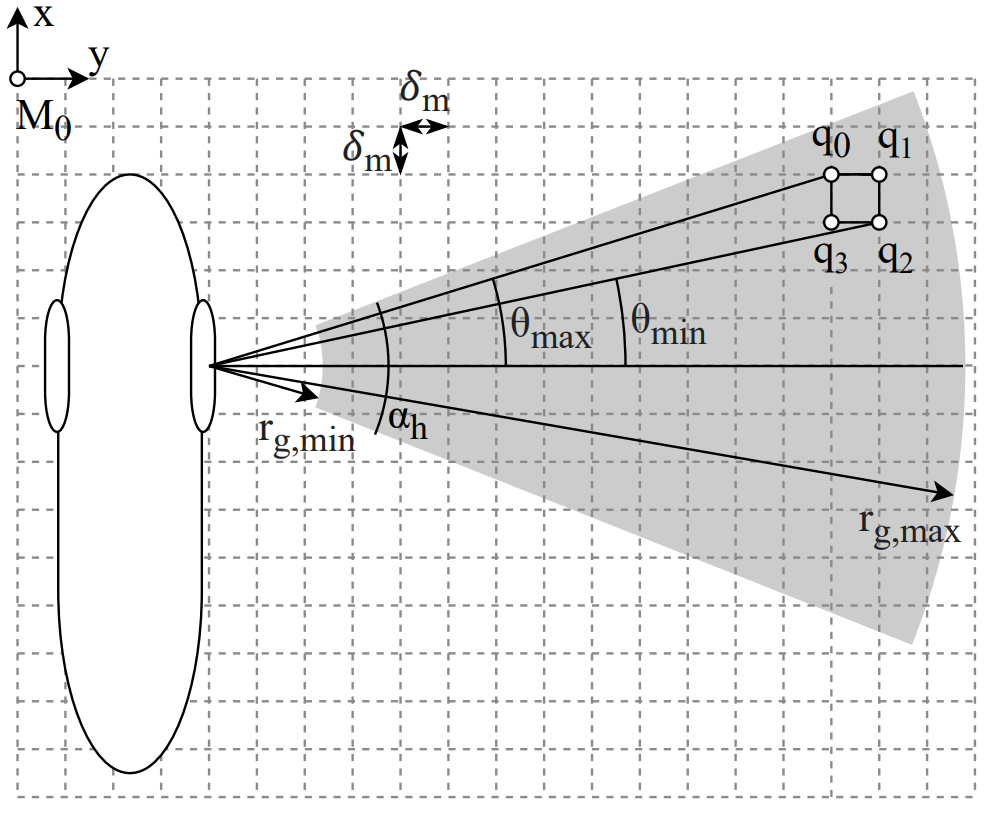
\includegraphics[width=0.70\linewidth]{Pictures/Local_Map_Generation/Map_Generation/Azimuth_Beam_Geometry.png}
    \caption{Top view illustration of the horizontal sonar beam geometry used during candidate measurement cell generation. For a single ping, candidate points are generated by sweeping outward in range from the corrected first bottom return boundary to the maximum usable range, while simultaneously sweeping across the horizontal beam sector of the transducer. This defines the continuous geometric footprint from which candidate map cells are later formed.\textsuperscript{\cite{side_scan_sonar_master_thesis}}}
    \label{fig:local-map-generation-candidate-cell-geometry}
\end{figure}
\noindent
For each pair $(r,\theta)$, a candidate illuminated point is first defined in the transducer frame as $\mathbf{p}_{q/t}^{t}(r,\theta)$, representing a possible seafloor point seen by the current ping. This point is then transformed into the body frame using the known transducer mounting pose,
\begin{equation}
    \mathbf{p}_{q/b}^{b} = \mathbf{R}_{t}^{b}\,\mathbf{p}_{q/t}^{t} + \mathbf{p}_{t/b}^{b}
    \label{eq:local-map-generation-cell-candidate-pose-in-body-frame}
\end{equation}
where $\mathbf{R}_{t}^{b}$ is the rotation from transducer frame to body frame and $\mathbf{p}_{t/b}^{b}$ is the transducer position relative to the body frame. Next, the candidate point is transformed from the body frame into the world or map frame using the current vehicle pose projected onto the horizontal plane,
\begin{equation}
    \mathbf{p}_{q/O}^{n} = \mathbf{R}_{b}^{n}\,\mathbf{p}_{q/b}^{b} + \mathbf{p}_{b/O}^{n}
    \label{eq:local-map-generation-cell-candidate-pose-in-map-frame}
\end{equation}
where $\mathbf{p}_{g/O}^{n}$ is the interpolated vehicle position and $\mathbf{R}_{b}^{n}$ is the corresponding body to world rotation restricted here to the local map plane. In this way, each sampled beam point is expressed directly in the same world referenced frame as the local map. This is the continuous map plane representation of the candidate illuminated point associated with the current ping. The earlier beam and roll geometry in Figure \ref{fig:local-map-generation-roll-correction} gives the related physical intuition for how this illuminated region is formed.
\\ \\
The resulting continuous point $\mathbf{p}_{q/O}^{n}$ is then discretized into a map cell index $q=(q_x,q_y)$ according to the map resolution $\delta_m$,
$$
    q_x = \mathrm{round}\!\left(\frac{x_q}{\delta_m}\right),
    \qquad
    q_y = \mathrm{round}\!\left(\frac{y_q}{\delta_m}\right)
$$
where $(x_q,y_q)$ are the horizontal coordinates of $\mathbf{p}_{q/O}^{n}$. This converts the continuous sonar footprint into discrete Cartesian cells that can be stored and reused in the following stages of the mapping algorithm.
\\ \\
If several sampled beam points fall into the same discrete map cell, they are merged immediately so that each cell is stored only once. The final result of this stage is therefore a sparse temporary candidate cell set for the current ping,
\begin{equation}
    Q_m = \left\{ q \;\middle|\; q \text{ is a discretized map cell reached by the current ping footprint} \right\}
    \label{eq:local-map-generation-qm-candidate}
\end{equation}
which serves as the geometric support for the following probabilistic weighting and intensity interpolation stages. The set is sparse because it contains only cells lying inside the currently illuminated sonar footprint rather than all cells of the dense local map, and it is temporary because it belongs only to the current processed swath and not yet to the final accumulated map.



\subsubsection{Probabilistic Pruning of Candidate Cells}
The candidate cell generation stage produces a large set of geometrically valid beam samples for each ping $Q_m$. However, if all of these samples were carried forward into the later interpolation and accumulation steps, the computational cost would quickly become too high, especially since many of the generated samples contribute only negligibly to the final map. A pruning stage is therefore introduced to reduce the candidate set before the more expensive mapping operations are performed. The goal of this step is to assign a beam based probability value to each candidate sample and reject those whose expected contribution is too small to matter in practice.
\\ \\
This pruning is performed in two stages. The first stage uses a very fast approximate beam probability, denoted by $P_m^{\mathrm{approx}}$, which is designed only for cheap early rejection. The second stage uses a more accurate probability, denoted by $P_m$, based on the integrated angular beam model. In this way, the majority of poor candidates can be removed using a lightweight approximation, while only the more promising candidates are evaluated using the more accurate but more expensive probabilistic model.
\\ \\
For a given sampled beam angle $\theta$ inside the horizontal sector, a normalized angular coordinate is first introduced as
$$
    u = \frac{\theta}{ \frac{\alpha_h}{2}}
$$
This expresses the current beam sample relative to the beam centerline, such that $u=0$ corresponds to the center of the beam and $|u|=1$ corresponds approximately to the beam edge. 
\\ \\
Using this normalized coordinate, a cheap center heavy approximation is defined as
\begin{equation}
    P_m^{\mathrm{approx}}(\theta) =
    \begin{cases}
        \left(1-u^2\right)^2, & |u| < 1 \\[0.25em]
        0, & |u| \geq 1
    \end{cases}
    \label{eq:local-map-generation-pm-approx}
\end{equation}
This approximation is strongest near the beam center and smoothly decreases toward the beam edges. It is not intended to be a physically exact beam model, but rather a very cheap way to reject obviously unimportant samples before spending more computation on them. If this approximate value falls below a predefined threshold,
$$
    P_m^{\mathrm{approx}}(\theta) < \varepsilon_{\mathrm{approx}}
$$
the candidate is removed immediately and is not carried forward. In practice, this first stage removes a large number of weak edge samples in $Q_m$ set at very low cost.
\\ \\
Only candidates surviving this first gate are evaluated using the more accurate probability model $P_m$. Here, the idea is that each sampled beam point represents not an infinitely thin ray, but a small angular interval whose width depends on both the map resolution and the current sampled range. If the sampled range is $r$, then the represented angular width is approximated by
$$
    \Delta \theta \approx \frac{\delta_m}{r}
$$
where $\delta_m$ is the map resolution. Thus, the current sample at angle $\theta$ is interpreted as covering the interval
$$
    \left[\theta - \frac{\Delta\theta}{2}, \, \theta + \frac{\Delta\theta}{2}\right]
$$
The horizontal beam is then modeled as a Gaussian angular distribution centered on the beam axis. Let
$$
    p(\varphi) = \mathcal{N}(0,\sigma^2),
    \qquad
    \sigma = \frac{\alpha_h}{2}
$$
denote this beam model in angle space. The probability assigned to the current candidate is then computed as the integrated Gaussian mass over the represented angular interval
$$
    P_m(\theta) =
    \int_{\theta - \frac{\Delta\theta}{2}}^{\theta + \frac{\Delta\theta}{2}} p(\varphi)\, d\varphi
$$
Equivalently, this may be evaluated using the Gaussian cumulative distribution function as
\begin{equation}
    P_m(\theta) =
    \Phi\!\left(\theta + \frac{\Delta\theta}{2}\right)
    -
    \Phi\!\left(\theta - \frac{\Delta\theta}{2}\right)
    \label{eq:local-map-generation-pm}
\end{equation}
where $\Phi(\cdot)$ denotes the CDF of the zero-mean Gaussian beam model. This gives a more physically meaningful probability than the approximate stage, since it accounts for the finite angular support represented by the candidate sample rather than only evaluating a simple pointwise weighting.
\\ \\
This accurate probability is then also used as a pruning criterion. If
$$
    P_m(\theta) < \varepsilon_{\mathrm{prob}}
$$
the candidate is discarded. Otherwise, it is retained and carried forward in the temporary map structure. In practice, $P_m$ is also stored together with the surviving candidate cell, since it will be needed later during the intensity accumulation stage and should therefore not be recomputed unnecessarily.
\\ \\
The reason for using this two-stage pruning strategy is that most invalid or negligible candidates can be rejected by the cheap approximation before the Gaussian based probability ever needs to be evaluated. This makes the pruning step both a physical modeling stage and a runtime optimization stage. The approximation provides speed, while the integrated Gaussian model provides a more meaningful measure of how strongly a candidate cell is illuminated by the current ping.
\\ \\
After the two pruning stages, the original candidate set $Q_m$ is reduced to a much smaller subset containing only the cells that are considered meaningful under the probabilistic beam model. In other words, the approximate probability $P_m^{\mathrm{approx}}$ and the accurate probability $P_m$ act together to redefine the temporary candidate support, cells with negligible contribution are removed, while only the physically relevant cells remain. The result is therefore a new pruned version of $Q_m$, now consisting only of candidate cells that are sufficiently likely to matter for the current ping.
\\ \\
At the same time, the corresponding probability values $P_m(q)$ for the surviving cells are kept and stored together with the pruned set. This is useful both physically and computationally. Physically, it means that the algorithm now has a compact set of map cells that are considered meaningfully illuminated by the sonar. Computationally, it means that both the reduced candidate set $Q_m$ and its associated probability values $P_m(q)$ can be reused in the later stages without recomputing the beam model again.
\\ \\
The overall result of this stage is therefore a sparse and much smaller probabilistic candidate support for the current ping, where only the relevant cells remain and each of them is already associated with its beam probability. This pruned support forms the basis for the following interpolation and map accumulation steps. An example of this retained probabilistic support is illustrated in Figure \ref{fig:local-map-generation-probability-map}, where the surviving candidate region appears as a structured illuminated subset of the local map rather than a dense full-grid representation.
\begin{figure}[H]
    \centering
    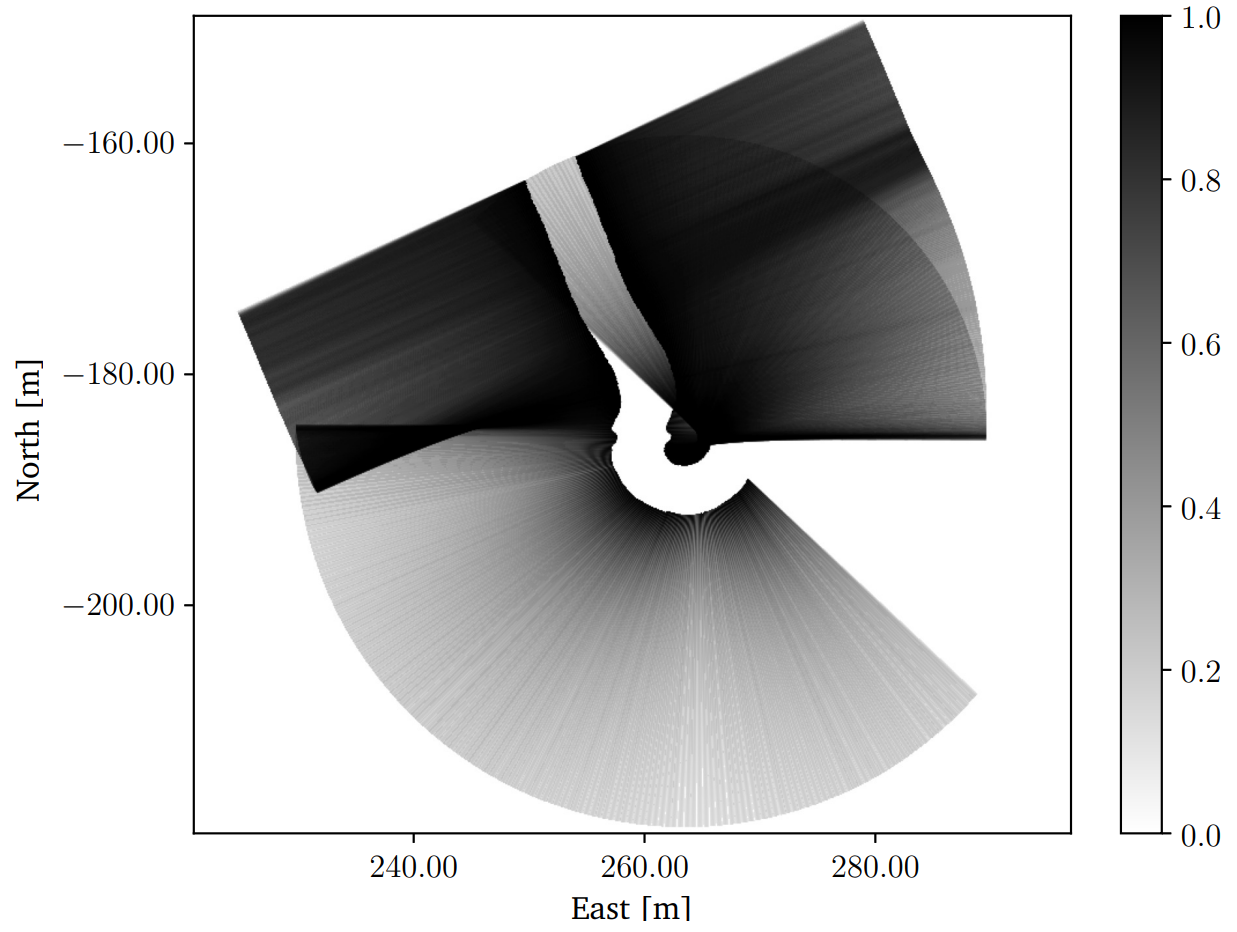
\includegraphics[width=1.00\linewidth]{Pictures/Local_Map_Generation/Map_Generation/Probabilistic_Map.png}
    \caption{Example visualization of probabilistic beam support in the local map. The image illustrates how candidate cells that survive the pruning stage retain nonzero beam probability values, while cells with negligible contribution are removed. Rather than representing the final fused map, this type of visualization is better interpreted as showing the spatial support created by the probabilistic beam model, which later guides intensity interpolation and map accumulation.\textsuperscript{\cite{side_scan_sonar_master_thesis}}}
    \label{fig:local-map-generation-probability-map}
\end{figure}



\newpage



\subsubsection{Interpolating the Intensity Measurement Map}
After probabilistic pruning, the surviving candidate set $Q_m$ contains only the map cells that are considered meaningfully illuminated by the current ping, and each such cell already carries an associated beam probability $P_m(q)$. However, these cells still need an intensity value from the processed sonar swath before they can contribute to the local map. The purpose of this stage is therefore to assign to each surviving candidate cell a representative intensity value, denoted by $V_m(q)$, by querying the processed swath only at those locations that have already been judged physically relevant. In this way, the algorithm first decides which map cells are plausible and only afterwards evaluates the sonar intensity for those cells, avoiding unnecessary interpolation over a large number of negligible candidates.
\\ \\
For each surviving map cell $q \in Q_m$, the corresponding map location is transformed back from the local map frame into the body frame and then into the transducer frame, that is, the same geometric relation used previously to generate the candidate point is now followed in the reverse direction in order to recover the sonar relative point $\mathbf{p}_{q/t}^{t}$. Thus, this stage effectively backprojects each surviving map cell into sonar slant range space, reusing the same geometric chain introduced in the candidate cell generation step in Equations \ref{eq:local-map-generation-cell-candidate-pose-in-body-frame} and \ref{eq:local-map-generation-cell-candidate-pose-in-map-frame}, now inverted so that the already selected map cells can be related directly to the processed swath.
\\ \\
Rather than using only the center of a map cell, the interpolation is performed using all four corners of the cell footprint. This is important because a finite map cell covers an area rather than a single point, and using only the center would make the sampled intensity more sensitive to discretization effects and local geometric mismatch. By evaluating all four corners and averaging the result, the assigned cell intensity becomes more stable and more representative of the full cell area.
\\ \\
Let the center of a surviving map cell $q \in Q_m$ be denoted by $\mathbf{p}_{q_c}^{n}$. Since each map cell has side length equal to the map resolution $\delta_m$, the distance from the cell center to any corner along each planar axis is $\delta_m/2$. The four cell corners are therefore obtained by adding all sign combinations of this half-cell offset to the center point, that is,
$$
    \mathbf{p}_{q_k}^{n}
    =
    \mathbf{p}_{q_c}^{n}
    +
    \frac{\delta_m}{2}
    \begin{bmatrix}
        s_{x,k} \\ s_{y,k}
    \end{bmatrix},
    \qquad
    s_{x,k}, s_{y,k} \in \{-1,+1\},
    \qquad
    k=1,\dots,4
$$
In other words, the factor $\delta_m/2$ gives the half-width of the cell, while the sign choices $s_{x,k}$ and $s_{y,k}$ determine whether the corner lies in the positive or negative direction along each planar axis. This compactly generates the four combinations corresponding to the four corners of the square cell. Each of these corners is then transformed back into the transducer frame, yielding the corresponding sonar relative corner positions.
$$
    \mathbf{p}_{q_k}^{t}, \qquad k=1,\dots,4
$$
From these sonar relative corner positions, the horizontal ground range distance of each corner is obtained as the planar norm
$$
    r_{g_k} = \left\| \mathbf{p}_{q_k}^{t} \right\|,
    \qquad k=1,\dots,4
$$
Using the corrected transducer height $h_t$ for the current channel, the corresponding slant range of each corner is then computed as
$$
    r_{s_k} = \sqrt{r_{g_k}^2 + h_t^2}
$$
Thus, each corner of the map cell is related back to a specific slant-range location in the processed swath. Since the processed swath is sampled only at discrete slant range intervals $\delta_s$, the intensity at the continuous range location $r_{s,k}$ must be obtained by interpolation between the two neighboring swath samples. The lower and upper neighboring sample locations are given by
$$
    \left\lfloor \frac{r_{s_k}}{\delta_s} \right\rfloor,
    \qquad
    \left\lceil \frac{r_{s_k}}{\delta_s} \right\rceil
$$
To interpolate smoothly between them, two weights are introduced. The first weight measures how far the continuous slant range position lies from the lower sample toward the upper one
$$
    w_{1_k}
    =
    \frac{r_{s_k}}{\delta_s}
    -
    \left\lfloor \frac{r_{s_k}}{\delta_s} \right\rfloor
$$
while the second weight is simply the complementary part
$$
    w_{2_k} = 1 - w_{1_k}
$$
In other words, if the corner lies close to the lower neighboring sample, then $w_{2_k}$ becomes dominant, while if it lies close to the upper neighboring sample, then $w_{1_k}$ becomes dominant. Using these two weights, the interpolated processed swath reflectivity at the corner slant range is obtained as
$$
    \hat{R}_m(r_{s_k})
    =
    w_{2_k}\,
    \hat{R}_m\!\left(
        \left\lfloor \frac{r_{s_k}}{\delta_s} \right\rfloor
    \right)
    +
    w_{1_k}\,
    \hat{R}_m\!\left(
        \left\lceil \frac{r_{s_k}}{\delta_s} \right\rceil
    \right)
$$
Thus, $\hat{R}_m(r_{s_k})$ is the linearly interpolated reflectivity value assigned to corner $k$ by blending the two nearest processed swath samples according to how close the corner lies to each of them. The four interpolated corner intensities are then combined into one representative cell intensity by simple averaging
\begin{equation}
    V_m(q) = \frac{1}{4}\sum_{k=1}^{4} \hat{R}_m(r_{s_k})
    \label{eq:local-map-generation-vm}
\end{equation}
This averaged value is the intensity measurement associated with the candidate cell $q$ for the current ping. Repeating this procedure for all surviving cells in $Q_m$ yields the temporary intensity map $V_m$, that is, the set of pruned candidate cells together with their associated interpolated reflectivity values. This is done separately for the port and starboard channels, since the two sides generally have different corrected transducer heights and transducer parameters, even though the same interpolation logic is used for both.



\subsubsection{Persistent Measurement State Accumulation}
After the candidate generation, probabilistic pruning, and intensity interpolation stages, the quantities $Q_m$, $P_m$, and $V_m$ describe only the current processed ping $m$. Here, $Q_m$ is the pruned set of candidate cells illuminated by that ping, $P_m(q)$ is the beam based probability assigned to each such cell, and $V_m(q)$ is the corresponding interpolated intensity measurement. However, the local map must represent the accumulated contribution from many pings rather than only the current one. The purpose of this stage is therefore to merge the temporary per ping quantities into persistent map states that are updated incrementally over time.
\\ \\
The persistent states are denoted by $Q$, $P$, and $V$. The set $Q$ represents the full accumulated set of map cells that have been meaningfully illuminated across all processed pings so far. The quantity $P(q)$ represents the accumulated observation probability of cell $q$, while $V(q)$ represents the accumulated probability weighted intensity of that same cell. Thus, $P$ stores how strongly and how often a cell has been supported by the beam model, while $V$ stores the corresponding accumulated weighted reflectivity contribution. At this stage, $V$ is not yet the final map intensity, but rather an intermediate weighted sum that will later be normalized by $P$.
\\ \\
Before the current ping contribution is inserted into the persistent map states, the temporary port and starboard measurement maps are first merged into one combined measurement map for the current swath. Since both sides are already expressed in the same map frame, this merge is performed cell wise. If a cell appears only in one channel, its values are copied directly. If the same discrete map cell appears in both port and starboard, then the common map location is kept and the two channel contributions are merged into a single temporary cell representation. In the present implementation, the strongest available probability and intensity values are retained for the overlapping cell, so that the current ping contributes only one entry per map cell even if both channels reach it.
\\ \\
Once this merged per ping measurement map has been formed, it is accumulated into the persistent map states. Conceptually, the persistent illuminated cell set is updated as the union
\begin{equation}
    Q \leftarrow Q \cup Q_m
    \label{eq:local-map-generation-q-accumulation}
\end{equation}
meaning that any cell reached by the current ping is added to the full accumulated illuminated support. For each cell $q \in Q_m$, the corresponding persistent probability state is updated by
\begin{equation}
    P(q) \leftarrow P(q) + P_m(q)
    \label{eq:local-map-generation-p-accumulation}
\end{equation}
and the persistent weighted intensity state is updated by
\begin{equation}
    V(q) \leftarrow V(q) + P_m(q)\,V_m(q)
    \label{eq:local-map-generation-v-accumulation}
\end{equation}
Thus, every new ping contributes both an additional probability mass and an additional probability weighted intensity contribution to the already accumulated map states.
\\ \\
This accumulation rule is repeated for every processed ping. Over time, the set $Q$ grows to represent all relevant illuminated map cells seen so far, while $P$ and $V$ store the cumulative support and weighted reflectivity contributions associated with those cells. In this way, the mapping process remains incremental, each ping contributes only a local update, yet the persistent states gradually build a richer and more stable representation of the observed seafloor.
\\ \\
It is important to note that at this stage the map still does not store the final normalized image intensity directly. Instead, each cell stores the accumulated probability $P(q)$ and the accumulated weighted intensity $V(q)$. This is deliberate, since it allows the final normalized map value to be formed later in a separate step from the relation between these two persistent states. In other words, the present stage is responsible only for building and updating the persistent measurement support, not yet for producing the final dense map image.



\subsubsection{Normalized Intensity Map Construction}
After the persistent map states have been accumulated, the final local map is obtained simply by normalizing the accumulated weighted intensity by the accumulated probability. Thus, for each map cell $q$, the constructed map intensity is defined as
\begin{equation}
    M(q) = \frac{V(q)}{P(q)}
    \label{eq:local-map-generation-m}
\end{equation}
Here, $P(q)$ represents the accumulated observation probability of cell $q$, while $V(q)$ represents the corresponding accumulated probability weighted intensity. Their ratio therefore gives the final normalized reflectivity value assigned to that cell. In this way, the map construction step converts the intermediate accumulated states into the final local grayscale map $M$, which is the representation used in the later stages of the pipeline.



\subsubsection{Fast Gap Filling Algorithm}
Even after the normalized intensity map $M$ has been constructed, small local holes can still remain. These gaps arise naturally from sparse sonar coverage, discretization onto the map grid, and the earlier aggressive pruning steps, where weak candidates are intentionally removed for both physical and computational reasons. As a result, the map may contain tiny empty cells inside otherwise well supported local regions.
\\ \\
To address this, a lightweight local gap filling algorithm is applied. The purpose of this step is not to reconstruct missing seafloor structure in a global sense, but only to repair small local discontinuities in already observed regions. A custom method is used because the goal here is fast, local, and conservative filling rather than general interpolation. In particular, the algorithm reuses the already available valid support structure from the sparse cached map state, so it only needs to iterate over spatially relevant cells instead of scanning the entire dense map repeatedly. This keeps the complexity much lower in practice than a full image iterative filling method. If the number of candidate empty cells is denoted by $N_e$ and the number of fill passes by $N_p$, the practical complexity is approximately
$$
    \mathcal{O}(N_p\,N_e)
$$
since each pass checks only the unresolved candidate cells and only over a fixed local neighborhood.
\\ \\
The algorithm first collects candidate empty cells only inside the active cached map regions. This is important because only these regions are relevant for filling, and empty cells far outside the observed support should not be considered at all. To do this efficiently, a temporary local occupancy mask is built for each active region. This mask simply records which local cells already contain valid map values and which are empty, making it possible to collect the fill candidates quickly without repeatedly querying the full sparse representation.
\\ \\
Once this candidate list has been formed, the algorithm performs a small number of iterative fill passes over only the currently unresolved empty cells. At the beginning of each pass, the current map is copied into a frozen source map. This means that any newly filled pixel in the current pass does not immediately affect the filling of other pixels in the same pass. Instead, all decisions within one pass are based only on the map state from the start of that pass, which makes the filling behavior more stable and predictable.
\\ \\
For each candidate empty cell, a local $3 \times 3$ neighborhood is examined. The cell is filled only if enough valid neighboring pixels are already present. If $N(q)$ denotes the set of valid neighbors of cell $q$, then the neighborhood support criterion can be written as
\begin{equation}
    |N(q)| \geq N_{\min}
    \label{eq:local-map-generation-gapfill-support}
\end{equation}
where $N_{\min}$ is the minimum required number of valid neighbors. If this condition is satisfied, the empty cell is assigned the local neighborhood average
\begin{equation}
    M(q) = \frac{1}{|N(q)|}\sum_{q' \in N(q)} M(q')
    \label{eq:local-map-generation-gapfill-update}
\end{equation}
If the support is insufficient, the cell is left unresolved and carried forward to the next pass.
\\ \\
This procedure continues iteratively until either the maximum number of passes has been reached or no new cells are filled during a pass. The latter gives the early stopping rule,
\begin{equation}
    N_{\mathrm{filled}} = 0 \;\Rightarrow\; \text{stop}
    \label{eq:local-map-generation-gapfill-stop}
\end{equation}
which avoids wasting computation when further passes would no longer change the result.
\\ \\
The overall result is a fast local repair step that fills only small holes inside already observed map regions. It is therefore best understood as a conservative refinement stage, it improves local continuity and visual consistency of the map, but it is not intended to invent large missing regions or extrapolate unsupported structure.



\subsubsection{Optimization and Memory-Compute Tradeoffs}
The map generation pipeline is dominated by repeated geometric transformations, probabilistic beam evaluation, sparse map updates, and local neighborhood operations. Without dedicated optimization, the computational cost would quickly become too high for real time execution, especially as more pings are processed and the local map grows over time. For this reason, the final implementation is built around a set of optimization strategies that do not change the underlying mapping model, but make it computationally practical on resource and real time constrained embedded systems.
\\ \\
A central part of this optimization is the chunked sparse map representation. Instead of storing the local map as one large always allocated dense grid, the map is partitioned into fixed size spatial chunks, and only chunks that actually contain meaningful measurements are allocated and updated. This is not only a storage trick, but a core algorithmic structure used throughout the entire map generation pipeline. The persistent states $Q$, $P$, and $V$ are therefore stored only where valid support exists, which means that later stages such as accumulation, dense reconstruction, and gap filling do not have to operate on the full theoretical map domain, but only on the active subset that has actually been observed.
\\ \\
For each newly processed ping, the surviving measurement cells are inserted into their corresponding spatial chunks. If a chunk is touched by a new measurement, it is either created if it does not already exist, or updated if it already contains data. At the same time, its age is reset to zero. Chunks that are not touched during a map update cycle are instead aged, and once their age exceeds a predefined threshold, they are removed. Conceptually, this can be written as
$$
    \text{age}_c \leftarrow 0 \quad \text{if chunk } c \text{ is updated},
    \qquad
    \text{age}_c \leftarrow \text{age}_c + 1 \quad \text{otherwise}
$$
with the pruning condition
$$
    \text{age}_c > \text{age}_{\max} \;\Rightarrow\; c \text{ is removed}
$$
This aging and pruning mechanism is essential, because it keeps the local map spatially bounded in practice, limits memory growth over long operation times, and ensures that the active map remains focused on the currently relevant region rather than expanding indefinitely. The corresponding behavior is illustrated in Figure \ref{fig:local-map-generation-chunk-aging}.
\begin{figure}[H]
    \centering
    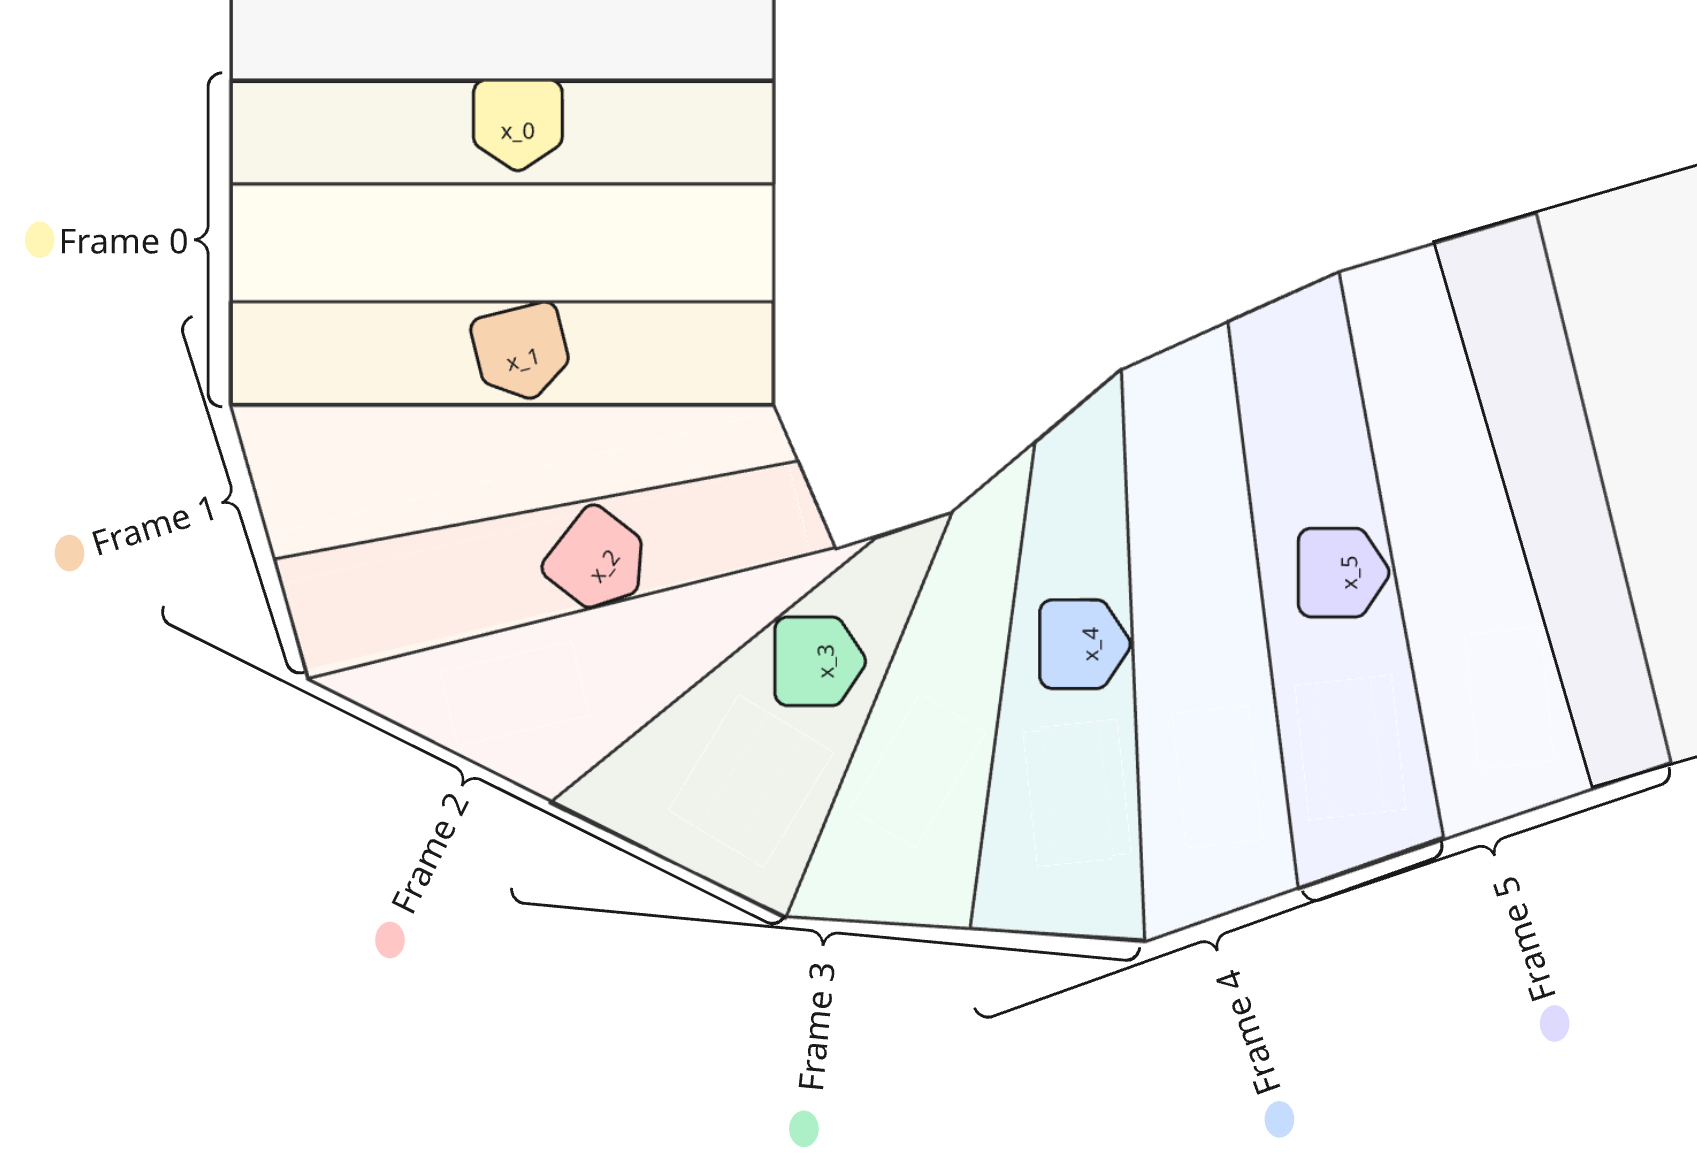
\includegraphics[width=0.9\linewidth]{Pictures/Local_Map_Generation/Map_Generation/Chunk_Map_Windows.png}
    \caption{Illustration of the sparse chunked local map with chunk aging and pruning over time. Chunks that receive new measurements remain active and have their age reset, recently visited chunks are retained temporarily, and old untouched chunks are eventually removed once they exceed the allowed age threshold. This keeps the local map spatially bounded and memory efficient while allowing continuity between successive map updates.}
    \label{fig:local-map-generation-chunk-aging}
\end{figure}
\noindent
This chunk structure also directly improves the runtime of the rest of the algorithm. Candidate accumulation updates only the touched chunks, dense map construction is performed only over the currently active chunk bounds, and the fast gap filling stage iterates only over empty cells inside active chunks. In this way, chunk management reduces both memory and computation simultaneously, since the algorithm never needs to process large regions of empty or outdated map space. At the same time, this representation also makes the map dynamic and flexible, because the spatial map can grow naturally as new chunks are touched rather than requiring a fixed predefined map size in advance. This means the algorithm can adapt to different operating environments and mission lengths without needing to redesign the map dimensions beforehand, which makes the overall method more scalable and easier to deploy across different systems.
\\ \\
A second major optimization is the use of pre-computation together with caching and selective online computation. The key idea is that the computational cost is not uniform throughout the full algorithm depth. Near the start of the pipeline, the number of possible evaluations is very large, so direct computation at that stage would be extremely expensive. In contrast, the memory cost of storing precomputed values is still relatively modest there. As the algorithm progresses deeper, however, the situation gradually reverses, the remaining candidate space becomes much smaller, so direct lookahead computation becomes cheaper, while precomputing and storing all deeper possibilities would make memory usage grow too much. The practical solution is therefore to precompute and cache useful information early, where the branching cost is highest, and then switch over to direct computation later, once the active set has already been sufficiently reduced.

\newpage

\noindent
This is where caching becomes important. When the same or similar intermediate quantities are needed repeatedly, the algorithm can reuse values already stored in memory instead of recomputing them from scratch. In practical terms, this gives cache hits, meaning that the required value is already available and can be retrieved at much lower cost than a fresh computation. Thus, caching links early pre-computation with later online execution and reduces the cost of repeated expensive operations.
\\ \\
This is fundamentally a time-space tradeoff, also called a time-memory tradeoff. The point is neither to memorize everything, since that would grow memory too much, nor to compute everything from scratch, since that would make the runtime too high. Instead, the practical balance is to combine partial pre-computation, cache reuse, and selective lookahead computation. The conceptual balance used in this work is illustrated in Figure \ref{fig:local-map-generation-time-space-tradeoff}.
\begin{figure}[H]
    \centering
    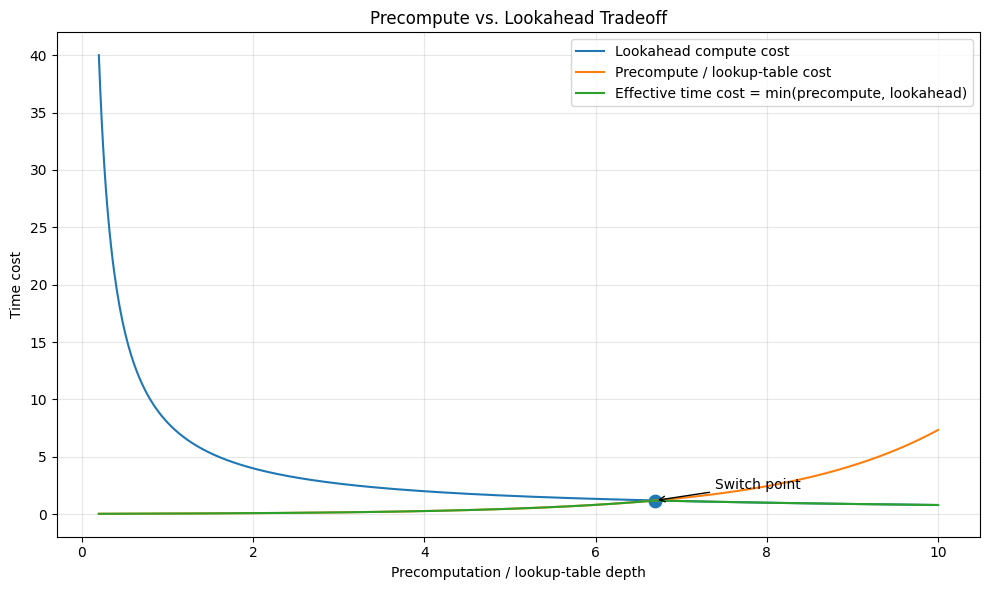
\includegraphics[width=0.9\linewidth]{Pictures/Local_Map_Generation/Map_Generation/Precompute_vs_Lookahead_Tradeoff.png}
    \caption{Conceptual illustration of the time-space tradeoff used in the map generation pipeline. Near the start of the algorithm, direct computation is expensive because many possible evaluations must be considered, while pre-computation is still relatively affordable. As the algorithm progresses deeper, the remaining candidate space becomes smaller, so direct lookahead computation becomes cheaper, whereas storing all deeper possibilities would make memory usage grow rapidly. The practical solution is therefore to use pre-computation early, reuse stored values through cache hits whenever possible, and then switch to direct online computation once the active candidate set has been reduced.}
    \label{fig:local-map-generation-time-space-tradeoff}
\end{figure}
\noindent
The same optimization philosophy appears throughout the full map generator. Two-stage probabilistic pruning reduces the number of candidate cells before expensive interpolation is performed. Sparse chunk storage keeps only active map support in memory. Gap filling operates only on candidate empty cells inside active regions. Dense reconstruction is delayed until a final map output is needed. Altogether, this shifts the implementation from an impractical exhaustive strategy toward a much more manageable regime,
$$
    \mathcal{O}(N_{\mathrm{all}})
    \;\longrightarrow\;
    \mathcal{O}(N_{\mathrm{active}}),
    \qquad
    N_{\mathrm{active}} \ll N_{\mathrm{all}}
$$
In this sense, the optimization strategy is one of the reasons the map generation pipeline remains feasible for real-time embedded operation. The final implementation is therefore best understood as a combination of sparse chunk management, bounded-memory aging and pruning, partial pre-computation, caching, selective local processing, and delayed dense reconstruction.



\newpage



\subsubsection{Optimized Algorithm}
The complete optimized map generation pipeline can now be summarized compactly. Starting from one processed ping, the algorithm first generates the candidate measurement support, then prunes this support probabilistically, assigns interpolated intensity measurements to the surviving cells, accumulates the resulting per ping contribution into the persistent map states, constructs the normalized local map, and finally applies a lightweight gap filling refinement.
\\ \\
In compact form, the optimized pipeline may therefore be written as
$$
    Q_m
    \;\xrightarrow{\text{Eq.\,\eqref{eq:local-map-generation-pm-approx},\,\eqref{eq:local-map-generation-pm}}}
    \{Q_m,P_m\}
    \;\xrightarrow{\text{Eq.\,\eqref{eq:local-map-generation-vm}}}
    V_m
    \;\xrightarrow{\text{Eq.\,\eqref{eq:local-map-generation-q-accumulation}--\eqref{eq:local-map-generation-v-accumulation}}}
    \{Q,P,V\}
    \;\xrightarrow{\text{Eq.\,\eqref{eq:local-map-generation-m}}}
    M
    \;\xrightarrow{\text{Eq.\,\eqref{eq:local-map-generation-gapfill-support}--\eqref{eq:local-map-generation-gapfill-stop}}}
    M_{\mathrm{filled}}
$$
Here, the candidate set $Q_m$ is first generated from the sonar footprint as defined in Equation \eqref{eq:local-map-generation-qm-candidate}. This temporary set is then reduced through the two-stage probabilistic pruning process, where the approximate beam model from Equation \eqref{eq:local-map-generation-pm-approx} performs the first fast rejection step and the more accurate beam probability from Equation \eqref{eq:local-map-generation-pm} determines the final retained support. For the surviving cells, the interpolated intensity measurement map $V_m$ is obtained from Equation \eqref{eq:local-map-generation-vm}. The resulting per ping quantities are then accumulated into the persistent map states through Equations \eqref{eq:local-map-generation-q-accumulation} to \eqref{eq:local-map-generation-v-accumulation}. After this accumulation, the normalized local reflectivity map is constructed from Equation \eqref{eq:local-map-generation-m}. Finally, the fast local gap filling refinement is applied using the support condition in Equation \eqref{eq:local-map-generation-gapfill-support}, the local fill update in Equation \eqref{eq:local-map-generation-gapfill-update}, and the stopping rule in Equation \eqref{eq:local-map-generation-gapfill-stop}.
\\ \\
The resulting final local map after probabilistic accumulation, normalization, and fast local gap filling is illustrated in Figure \ref{fig:local-map-generation-probabilistic-map}.
\begin{figure}[H]
    \centering
    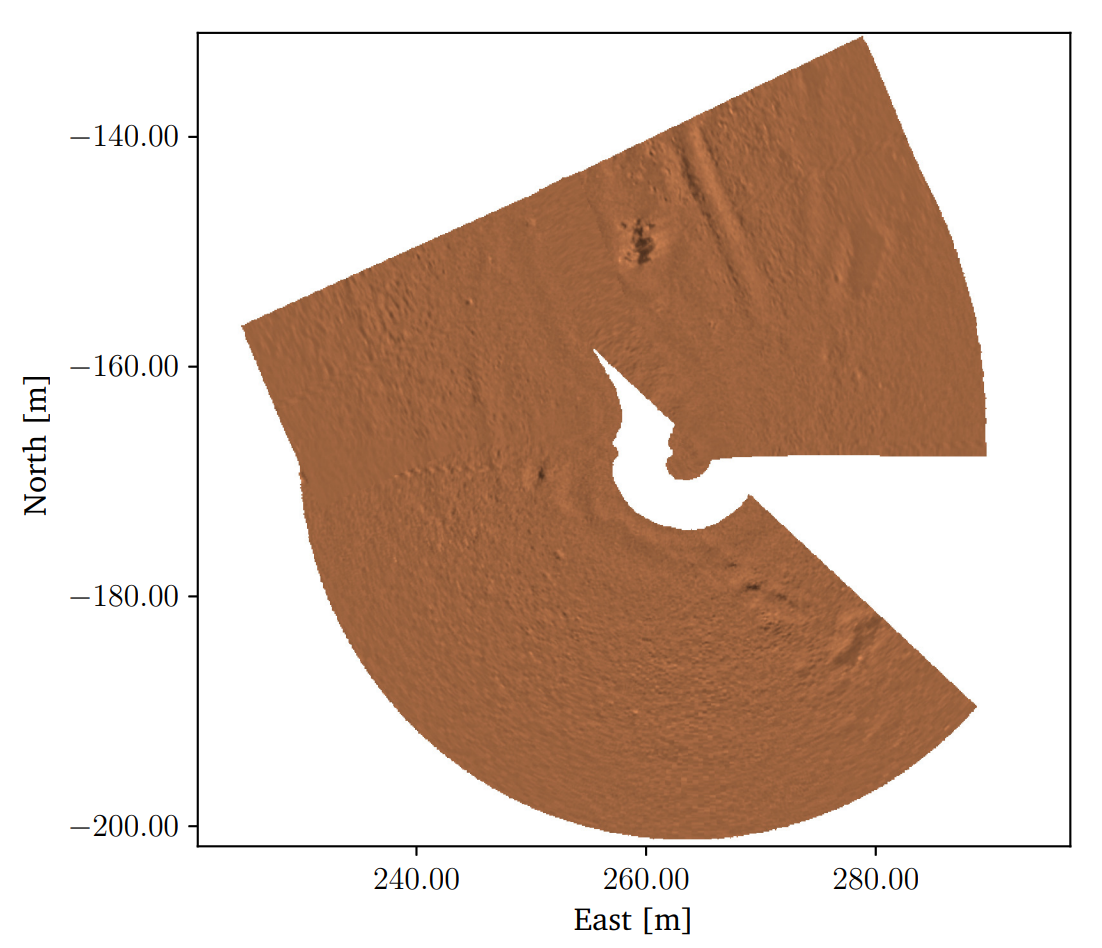
\includegraphics[width=0.85\linewidth]{Pictures/Local_Map_Generation/Map_Generation/Map.png}
    \caption{Final local reflectivity map produced by the optimized map generation pipeline after probabilistic accumulation, normalization, and fast local gap filling. This is the final dense map representation used in the later stages of the SLAM pipeline.\textsuperscript{\cite{side_scan_sonar_master_thesis}}}
    \label{fig:local-map-generation-probabilistic-map}
\end{figure}
